% Provenance (never printed): old terminale S material on the continental crust
% (granitic composition, thickness, density, age; roots and isostasy). Thickness
% from Christensen-Mooney 1995 and Cogley 1984 (CRUST1.0 dropped: no licence,
% Sync 1); ocean-floor ages from figdata/grade-12/crust_ages.py (Seton 2020 grid,
% as in g11.01). Airy isostasy is g11.03's: recalled, not re-derived. Radiometric
% dating is g12.07's: ages are only quoted here.
\chapter{القشرة القارية}\label{ch:g12:continental-crust}

في شمال غرب كندا، قرب نهر أكاستا، يتكشف صخر رمادي
مخطط بأشرطة فاتحة وداكنة. وقد أُرِّخ بما بين 4.00 و4.03 مليار
سنة: إنه نيس أكاستا، أقدم صخر معروف. وأقدم منه حبيبات
معدن الزركون، طول كل منها جزء من المليمتر، وُجدت في صخور
رسوبية قديمة في تلال جاك في غرب أستراليا. فقد تآكلت من صخور أقدم
وحملها الماء قبل أن تُدفن، وكانت قد تبلورت قبل 4.4
مليار سنة، وهي تُظهر أن قشرة كانت موجودة حينئذ. ولا يبلغ عمر أي قاع محيطي حتى جزءًا من عشرين من ذلك. يسأل هذا الفصل
مِمَّ تتكون القارات، ولماذا تدوم.
% ledger: bowring99:acasta, wilde01:zircon, uw14:jack-hills, photo:g12-acasta, photo:g12-jack-hills-zircons

\begin{omfigure}
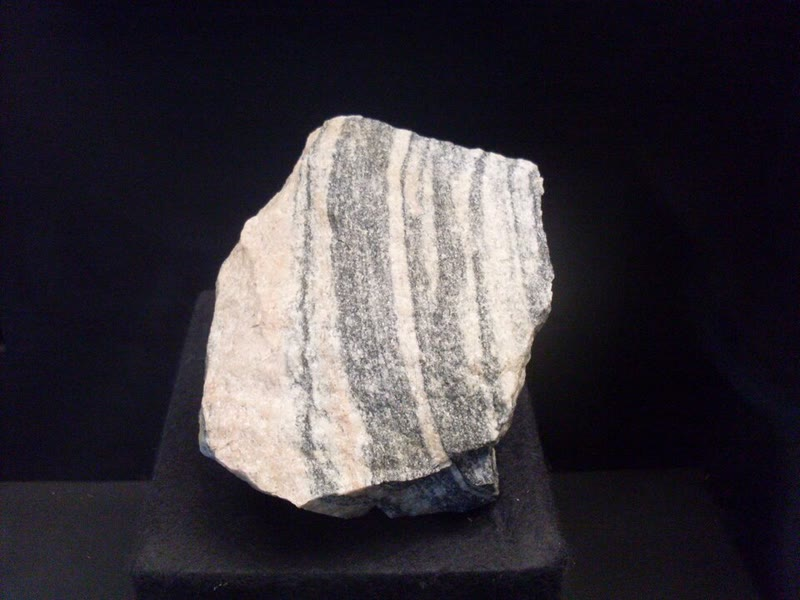
\includegraphics[height=4.6cm]{images/book2/g12-pedro-acasta-gneiss.jpg}\hspace{0.04\linewidth}%
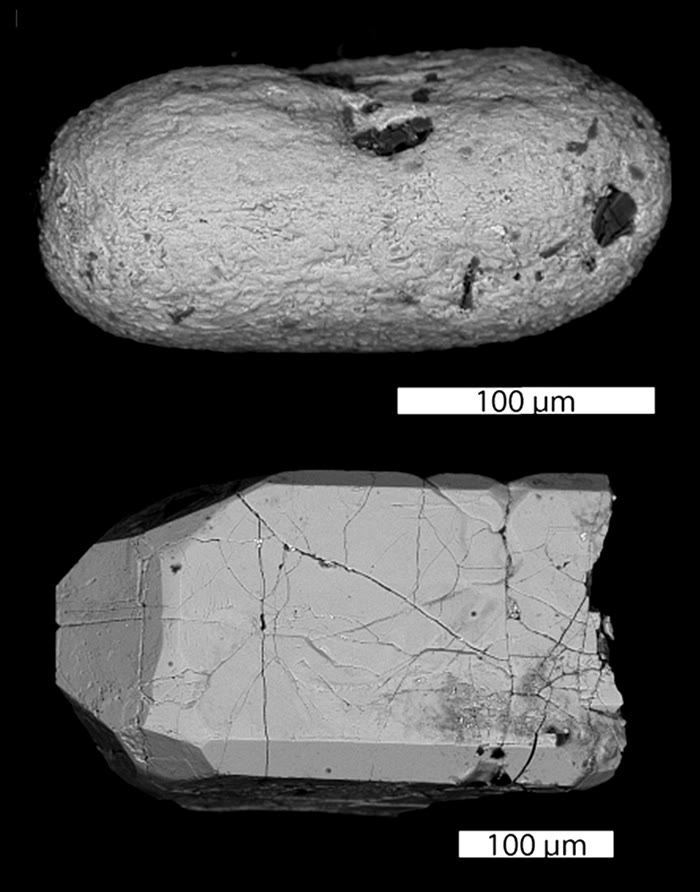
\includegraphics[height=4.6cm]{images/book2/g12-cavosie-jack-hills-zircons.jpg}

{\small في اليمين: قطعة من نيس أكاستا، عمرها 4.03 مليار سنة، في
معرض متحفي. الصورة: بيدرو ألكسندر أندرادي (\babelsublr{CC~BY-SA~3.0}). في اليسار: حبتا
زركون من تلال جاك، غرب أستراليا، تحت المجهر
الإلكتروني؛ وطول كل مسطرة قياس \qty{100}{\micro m}. وقد استدارت الحبة العليا
إذ حملها الماء، واحتفظت السفلى بأوجه بلورتها.
الصور: أ.~كافوسي وج.~فالي (ملك عام).}
\end{omfigure}
% ledger: photo:g12-acasta, photo:g12-jack-hills-zircons

\begin{recall}
تنتهي القشرة عند \omterm{def:g11:seismic-structure:moho}{الموهو}، الذي يقع تحته الوشاح الأكثف
(\cref{ch:g11:seismic-structure}). \omterm{def:g11:ocean-ridges:oceanic-lithosphere}{والقشرة المحيطية} نحو \qty{7}{km} من
البازلت \omterm{def:g11:ocean-ridges:gabbro}{والغابرو} تُصنع عند الظهرات (\cref{ch:g11:ocean-ridges})، ولا يتجاوز عمرها
أبدًا نحو 190 مليون سنة (\cref{ch:g11:drift-to-spreading}).
والطبقات الخارجية تطفو على الغلاف الموري: ففي نموذج إيري، المنطقة التي
ترتفع بمقدار $h$ أكثر تكون قشرتها أسمك بمقدار $h\,\rho_m/(\rho_m -
\rho_c)$ (\cref{ch:g11:lithosphere-asthenosphere}). وتُسمّى الصخور النارية
بحسب \omterm{def:g11:igneous-rocks:texture}{نسيجها} ومحتواها من السيليكا: \omterm{def:g11:igneous-rocks:felsic-mafic}{مافية} من 45 إلى
\qty{55}{\percent} من \ce{SiO2}، ومتوسطة من 55 إلى 65، \omterm{def:g11:igneous-rocks:felsic-mafic}{وفلسية} من 65 إلى
75 (\cref{ch:g11:igneous-rocks}). والعناصر المشعة تتفكك بمعدل
ثابت، وهذا ما يعطي الصخور أعمارها (كتب الفيزياء؛
\cref{ch:g12:age-of-the-earth}).
\end{recall}
% ledger: white92:crust, data:b2-seafloor-age, tulane:magma-types

\section{مِمَّ تتكون القارات}

\begin{definition}[القشرة القارية]\label{def:g12:continental-crust:continental-crust}
\emph{القشرة القارية}\index{قشرة قارية} هي القشرة التي
تكوّن القارات، بما فيها أجزاؤها الواقعة تحت البحار الضحلة. وهي
سميكة، غرانيتية التركيب في المتوسط في جزئها العلوي، خفيفة، ويمكن
أن تكون قديمة جدًا.
\end{definition}
% ledger: tulane:crust-types, tulane:roots, cogley84:continents

القارات أوسع من اليابسة. فحواف \omterm{def:g12:continental-crust:continental-crust}{القشرة القارية}
تقع تحت البحر، على الأرصفة القارية: وإذا رُسمت خريطتها على هذا النحو، فإن
\omterm{def:g12:continental-crust:continental-crust}{القشرة القارية} تغطي \num{210}~مليون~\unit{km^2}، أي \qty{41}{\percent} من
سطح الأرض، وثلثها تقريبًا، \qty{30.6}{\percent}، مغمور. وإذا
حُسبت مع أجزائها المغمورة، لم يتجاوز متوسط ارتفاع \omterm{def:g12:continental-crust:continental-crust}{القشرة
القارية} نحو \qty{120}{m} فوق مستوى سطح البحر.
% ledger: cogley84:continents

تُظهر القارات على سطحها كل أنواع الصخور --- الرسوبيات،
\omterm{def:g11:igneous-rocks:volcanic-plutonic}{والصخور البركانية}، والصخور المتحولة --- لكن \omterm{def:g12:continental-crust:continental-crust}{القشرة القارية} تحت الغطاء الرسوبي
تتكون في معظمها من صخور غرانيتية ومن الصخور المتحولة
والجوفية \omterm{def:g12:continental-crust:root}{لجذور جبال} قديمة. وفي المتوسط، تحوي \omterm{def:g12:continental-crust:continental-crust}{القشرة القارية} كلها
\qty{60.6}{\percent} من السيليكا؛ وجزؤها العلوي أغنى،
\qty{66.6}{\percent}، فلا بد أن يكون جزؤها الأعمق أفقر.
% ledger: rg14:crust, tulane:crust-types, cm95:crust

\begin{omfigure}
\begin{tikzpicture}
\begin{axis}[omrecord, ybar=0pt, width=0.92\linewidth, height=5.0cm, bar width=7pt,
  ymin=0, ymax=80, ylabel={\foreignlanguage{arabic}{الكسر الكتلي \babelsublr{(\unit{\percent})}}},
  symbolic x coords={SiO2, Al2O3, FeO, MgO, CaO, Na2O, K2O},
  xticklabels={\ce{SiO2}, \ce{Al2O3}, \ce{FeO}, \ce{MgO}, \ce{CaO}, \ce{Na2O}, \ce{K2O}},
  xtick=data, enlarge x limits=0.08, ymajorgrids=true, xmajorgrids=false,
  legend style={font=\scriptsize, at={(0.98,0.97)}, anchor=north east, legend columns=1}]
% ledger: rg14:crust (upper and bulk continental crust; FeO* total iron)
\addplot[fill=omLithGranite, draw=black!60] coordinates {(SiO2,66.6) (Al2O3,15.4) (FeO,5.04) (MgO,2.48) (CaO,3.59) (Na2O,3.27) (K2O,2.80)};
\addplot[fill=omProp!55, draw=black!60] coordinates {(SiO2,60.6) (Al2O3,15.9) (FeO,6.71) (MgO,4.66) (CaO,6.41) (Na2O,3.07) (K2O,1.81)};
% ledger: earle:magma-oxides (mafic magma: midpoint of each range, the bar spans the range)
\addplot[fill=omLithBasalt, draw=black!60, error bars/.cd, y dir=both, y explicit]
  coordinates {(SiO2,50) +- (0,5) (Al2O3,16) +- (0,2) (FeO,10) +- (0,2) (MgO,7) +- (0,2) (CaO,9) +- (0,2) (Na2O,2) +- (0,1) (K2O,1.75) +- (0,1.25)};
\legend{القشرة القارية العليا, القشرة القارية كلها, مدى الصهارة المافية}
\end{axis}
\end{tikzpicture}

{\small تركيب \omterm{def:g12:continental-crust:continental-crust}{القشرة القارية} مقارنةً بصهارة \omterm{def:g11:igneous-rocks:felsic-mafic}{مافية}، من
النوع الذي يصنع \omterm{def:g11:ocean-ridges:oceanic-lithosphere}{القشرة المحيطية}: الأكاسيد الرئيسية، بالنسبة المئوية من الكتلة
(يُحسب في \ce{FeO} كل الحديد). \omterm{def:g12:continental-crust:continental-crust}{القشرة القارية} أغنى بالسيليكا
والصوديوم والبوتاسيوم، وأفقر بالحديد والمغنيسيوم والكالسيوم. البيانات: رودنيك
وغاو (2014)؛ ومدى الصهارة \omterm{def:g11:igneous-rocks:felsic-mafic}{المافية} من س.~إيرل، \emph{الجيولوجيا الفيزيائية}
(\babelsublr{CC~BY~4.0}).}
\end{omfigure}
% ledger: rg14:crust, earle:magma-oxides

\section{قشرة سميكة وخفيفة}

تجد المسوح الزلزالية \omterm{def:g11:seismic-structure:moho}{الموهو} تحت القارات على أعماق شديدة
التباين. فإذا أُخذ المتوسط على كل القارات، موزونًا بالمساحة، كان سمك القشرة نحو
\qty{41}{km}؛ وهي أرق، نحو \qty{30}{km}، حيث
تمططت القشرة، وأسمك، نحو \qty{46}{km} في المتوسط، في الأحزمة الجبلية.
وبعيدًا عن الأحزمة الجبلية يبلغ سمكها عادةً من 35 إلى \qty{40}{km}؛ وتحت
أعلى السلاسل، من 50 إلى \qty{70}{km}، ونحو \qty{70}{km} تحت أجزاء من التبت.
\omterm{def:g11:ocean-ridges:oceanic-lithosphere}{والقشرة المحيطية} سمكها نحو \qty{7}{km}: \omterm{def:g12:continental-crust:continental-crust}{فالقشرة القارية} أسمك منها بخمس
إلى عشر مرات.
% ledger: cm95:crust, tulane:roots, karplus:tibet-moho, white92:crust

\begin{omfigure}
\begin{tikzpicture}
\begin{axis}[omrecord, xbar, bar shift=0pt, width=0.78\linewidth, height=5.0cm, bar width=8pt,
  xmin=0, xmax=80, ymin=0.4, ymax=5.6, ytick={1,...,5},
  yticklabels={القشرة المحيطية, {القارات المتمططة}, {متوسط القارات}, {متوسط الأحزمة الجبلية}, {تحت التبت}},
  xlabel={\foreignlanguage{arabic}{سمك القشرة \babelsublr{(\unit{km})}}}, ymajorgrids=false,
  nodes near coords, nodes near coords style={font=\scriptsize, anchor=west}, point meta=explicit symbolic]
% ledger: white92:crust, cm95:crust, karplus:tibet-moho
\addplot[fill=omLithBasalt, draw=black!60] coordinates {(7.1,1) [7.1]};
\addplot[fill=omLithGranite, draw=black!60] coordinates {(30.5,2) [30.5] (41.1,3) [41.1] (46.3,4) [46.3] (70,5) [نحو 70]};
\end{axis}
\end{tikzpicture}

{\small سمك القشرة من القياسات الزلزالية. البيانات: وايت
وماكنزي وأونيونز (1992) \omterm{def:g11:ocean-ridges:oceanic-lithosphere}{للقشرة المحيطية}؛ وكريستنسن وموني
(1995) للمتوسطات القارية؛ وكاربلس وآخرون (2019) للتبت.}
\end{omfigure}
% ledger: white92:crust, cm95:crust, karplus:tibet-moho

\omterm{def:g12:continental-crust:continental-crust}{والقشرة القارية} خفيفة أيضًا. فمتوسط كثافتها نحو
\qty{2830}{kg/m^3}. أما بازلت \omterm{def:g11:ocean-ridges:oceanic-lithosphere}{القشرة المحيطية} وغابروها، الغنيان
بالبيروكسين والأوليفين، فيبلغان نحو \qty{3000}{kg/m^3}
(\cref{ch:g11:minerals})، والوشاح الواقع تحت \omterm{def:g11:seismic-structure:moho}{الموهو} مباشرة نحو
\qty{3380}{kg/m^3}. والقشرة السميكة الخفيفة تطفو عاليًا: ولهذا تقف
القارات فوق قاع المحيط، ولهذا لا يمكن أن تُسحب قارة
إلى الأسفل في \omterm{def:g11:subduction-zones:subduction}{نطاق اندساس}. فحيث تصل قارة إلى خندق، تكون أخف من
أن تغوص؛ فيتوقف \omterm{def:g11:subduction-zones:subduction}{الاندساس}، وتتصادم القارتان
(\cref{ch:g12:mountain-building}). \omterm{def:g12:continental-crust:continental-crust}{والقشرة القارية}، ما إن تُصنع، يصعب
تدميرها.
% ledger: cm95:crust, data:prem, tulane:roots, tulane:no-subduct
% values (mineral_density.py): basalt/gabbro rock line 3.0015 g/cm3

\begin{omfigure}
\begin{tikzpicture}[x=1cm, y=0.075cm, font=\footnotesize]
  % continental column: 41 km of crust, surface at +0.12 km (mean height); ocean column: 3.7 km of water drawn schematically
  \fill[omLithGranite] (0,0) rectangle (3,-41);
  \fill[omLithPeridotite!60] (0,-41) rectangle (3,-60);
  \fill[omSea] (6,0) rectangle (9,-4);
  \fill[omLithGabbro] (6,-4) rectangle (9,-11.1);
  \fill[omLithPeridotite!60] (6,-11.1) rectangle (9,-60);
  \draw[black!60] (0,0) rectangle (3,-60) (6,0) rectangle (9,-60);
  \draw[line width=0.9pt] (0,-41) -- (3,-41) (6,-11.1) -- (9,-11.1);
  \node[align=center] at (1.5,-20) {قشرة قارية\\\foreignlanguage{arabic}{نحو \babelsublr{\qty{41}{km}}}\\\babelsublr{\qty{2830}{kg/m^3}}\\\foreignlanguage{arabic}{حتى 4 مليارات سنة}};
  \node[align=center] at (7.5,-24) {وشاح\\\babelsublr{\qty{3380}{kg/m^3}}\\تحت الموهو};
  \node[align=center] at (1.5,-50.5) {وشاح};
  \node at (7.5,-2) {محيط};
  \draw[black!60] (8.6,-7.6) -- (9.3,-7.6);
  \node[anchor=west, align=left] at (9.3,-7.6) {\foreignlanguage{arabic}{قشرة محيطية، نحو \babelsublr{\qty{7}{km}}}\\\babelsublr{\qty{3000}{kg/m^3}}\\\foreignlanguage{arabic}{أقل من 200 مليون سنة}};
  \node[anchor=east] at (-0.1,-41) {الموهو};
  \node[anchor=east] at (5.9,-11.1) {الموهو};
  \node[anchor=south] at (1.5,0) {قارة};
  \node[anchor=south] at (7.5,0) {محيط};
  \foreach \d in {0,20,40,60} {\draw[black!60] (-1.5,-\d) -- (-1.3,-\d); \node[anchor=east, font=\scriptsize] at (-1.5,-\d) {\d};}
  \draw[black!60] (-1.4,0) -- (-1.4,-60);
  \node[rotate=90, font=\scriptsize] at (-2.3,-30) {\foreignlanguage{arabic}{العمق \babelsublr{(\unit{km})}}};
\end{tikzpicture}

{\small قارة ومحيط جنبًا إلى جنب (الأعماق بمقياس رسم حقيقي، والعروض لا؛
والمحيط مرسوم بعمق \qty{4}{km}): \omterm{def:g12:continental-crust:continental-crust}{القشرة القارية} أسمك وأخف
وأقدم بكثير من \omterm{def:g11:ocean-ridges:oceanic-lithosphere}{القشرة المحيطية}.}
\end{omfigure}
% ledger: cm95:crust, white92:crust, data:prem, bowring99:acasta, data:b2-seafloor-age

\begin{method}[مقارنة القشرة القارية بالقشرة المحيطية]\label{met:g12:continental-crust:compare}
لمعرفة نوع القشرة الواقعة تحت مكان ما، قارن خمس خصائص:
\begin{enumerate}
  \item السمك: نحو \qty{7}{km} \omterm{def:g11:ocean-ridges:oceanic-lithosphere}{للقشرة المحيطية}، ومن 30 إلى
        \qty{70}{km} \omterm{def:g12:continental-crust:continental-crust}{للقشرة القارية}؛
  \item الصخور: البازلت \omterm{def:g11:ocean-ridges:gabbro}{والغابرو}، أو الغرانيت والنيس وما يشبههما،
        تحت غطاء من الرسوبيات؛
  \item التركيب: نحو \qty{50}{\percent} من السيليكا، أو نحو 60
        وأكثر؛
  \item الكثافة: نحو \qty{3000}{kg/m^3}، أو نحو \qty{2830}{kg/m^3}؛
  \item العمر: أقل من 200 مليون سنة، أو حتى 4 مليارات سنة.
\end{enumerate}
والارتفاع قرينة لا اختبار: فمعظم قاع المحيط يقع على عمق
كيلومترات، لكن حواف القارات تقع تحت بحار ضحلة.
\end{method}
% ledger: white92:crust, cm95:crust, rg14:crust, earle:magma-oxides, cogley84:continents

\begin{example}[قاع بحر ضحل]\label{ex:g12:continental-crust:shelf}
تجد سفينة مسح قاع بحر على عمق \qty{150}{m}. وتضع المقاطع الزلزالية
\omterm{def:g11:seismic-structure:moho}{الموهو} على عمق \qty{32}{km} تحت قاع البحر؛ ويأتي لب حفر، من تحت
الرسوبيات، بصخر خشن الحبيبات من الكوارتز والفلسبار والميكا. فأي قشرة
تقع هناك؟

\emph{الحل.} السمك نحو \qty{32}{km}: قارية، أرق من
المتوسط، كما هي حيث تمططت. وغرانيت تحت الرسوبيات:
قارية. فقاع البحر رصيف قاري، أحد الأجزاء المغمورة
التي تشكّل ثلث القارات تقريبًا.
\end{example}
% invented numbers; ledger: cm95:crust, cogley84:continents

ما وزن كل هذه القشرة؟ للطبقة الرقيقة مقارنةً بنصف قطر الأرض
كتلة بسيطة.

\begin{proposition}[كتلة طبقة رقيقة]\label{prop:g12:continental-crust:thin-layer}
طبقة سمكها $H$ وكثافتها $\rho$ تغطي كسرًا $f$ من
سطح كوكب نصف قطره $R \gg H$ ومتوسط كثافته $\bar\rho$، كتلتها
$m \approx 4\pi R^2 f H \rho$، وحصتها من كتلة الكوكب $M$ هي
\[
  \frac{m}{M} \approx 3 f\,\frac{H}{R}\,\frac{\rho}{\bar\rho}.
\]
\end{proposition}
% ledger: earth:Rmean, earth:density

\begin{proof}
مساحة سطح الكوكب $4\pi R^2$؛ والطبقة تغطي $4\pi R^2 f$،
ولأنها رقيقة فحجمها قريب من تلك المساحة مضروبةً في $H$، فإن $m \approx 4\pi R^2
f H \rho$. وكتلة الكوكب $M = \tfrac{4}{3}\pi R^3 \bar\rho$. وبالقسمة،
$m/M \approx 4\pi R^2 f H \rho / (\tfrac{4}{3}\pi R^3 \bar\rho) = 3 f (H/R)
(\rho/\bar\rho)$.
\end{proof}

بالنسبة إلى \omterm{def:g11:ocean-ridges:oceanic-lithosphere}{القشرة المحيطية} --- وهي تغطي \qty{59}{\percent} الباقية من السطح،
و\qty{7.1}{km}، ونحو \qty{3000}{kg/m^3} --- ومع $R = \qty{6371}{km}$
و$\bar\rho = \qty{5513}{kg/m^3}$، تكون الحصة $3 \times 0.59 \times
(7.1/6371) \times (3000/5513) \approx 0.0011$: أي نحو عُشر في المئة من
كتلة الأرض. ومسألة نهاية الأسبوع تفعل الشيء نفسه للقارات.
% ledger: cogley84:continents, white92:crust, earth:Rmean, earth:density

\section{قشرة قديمة}

قاع المحيط فتيّ في كل مكان: فثلاثة أرباعه أحدث من
100 مليون سنة، ولا يكاد شيء منه يتجاوز 190 مليون سنة. أما
القارات فأمر آخر. فصخورها تمتد على تاريخ الأرض كله تقريبًا،
من نيس أكاستا، الذي يبلغ عمره 4.03 مليار سنة، إلى اللابات المنبثقة
اليوم، وتحمل حبيبات الزركون السجل إلى الوراء حتى 4.4 مليار سنة.
% ledger: data:b2-seafloor-age, bowring99:acasta, uw14:jack-hills

\begin{omfigure}
\begin{tikzpicture}
\begin{axis}[omrecord, ybar interval, width=0.82\linewidth, height=5.0cm,
  xmin=0, xmax=200, ymin=0, ymax=0.12, xtick={0,20,...,200},
  xlabel={\foreignlanguage{arabic}{عمر قاع المحيط بملايين السنين}},
  ylabel={حصة من قاع المحيط}, yticklabel style={/pgf/number format/fixed},
  ymajorgrids=true, xmajorgrids=false, clip=false, x tick label as interval=false]
% computed in figdata/grade-12/crust_ages.py (Seton 2020 grid, 1-degree cells, area-weighted)
\addplot[fill=omDef!35, draw=omDef] table[x=age_lo, y=share] {figdata/out/grade-12-crust_ages-hist.dat};
\node[anchor=north east, align=right, font=\scriptsize, fill=white, inner sep=2pt] at (axis cs:198,0.115)
  {\foreignlanguage{arabic}{أقدم صخر قاري: \babelsublr{\num{4030}} مليون سنة،}\\أقدم من أقدم قاع محيطي بعشرين مرة};
\end{axis}
\end{tikzpicture}

{\small كم عمر قاع المحيط: حصة مساحته في كل شريط من 10
ملايين سنة. القاع الفتي هو الغالب؛ ولا يكاد شيء يتجاوز 190
مليون سنة (مع استبعاد بضعة أحواض قديمة في شرق البحر المتوسط).
البيانات: سيتون وآخرون (2020)، محسوبة.}
\end{omfigure}
% ledger: data:b2-seafloor-age, bowring99:acasta
% values (crust_ages.py): oldest_open_myr 192.5, share_younger_100 0.765, share_younger_150 0.956, rock_over_floor 20.9

تشكّل أقدم أجزاء القارات نواها.

\begin{definition}[الكراتون]\label{def:g12:continental-crust:craton}
\emph{الكراتون}\index{كراتون} نواة قديمة مستقرة لقارة:
\omterm{def:g12:continental-crust:continental-crust}{قشرة قارية} تكوّنت وتشوهت قبل أكثر من مليار سنة، ثم
بردت منذئذ ولم تعد تتشوه. وصخوره في معظمها صخور متحولة
وجوفية، هي \omterm{def:g12:continental-crust:root}{الجذور العميقة} لجبال سابقة.
\end{definition}
% ledger: tulane:cratons

تحيط بالكراتونات أحزمة من صخور مشوهة أحدث، هي \omterm{def:g12:continental-crust:root}{الجذور المتآكلة}
لسلاسل جبلية بُنيت لاحقًا؛ وتميل الأحزمة إلى أن تكون أحدث نحو حواف
القارة. فقد نمت القارة ببناء الجبال الذي لحم قشرة جديدة
بحوافها، حول نواة قديمة. وفي كندا، حيث تقع صخور \omterm{def:g12:continental-crust:craton}{الكراتون}
على السطح، تتكشف صخور من النيس والغرانيت يتراوح عمرها بين 1 و3 مليارات سنة،
كما هنا على شاطئ بحيرة.
% ledger: tulane:cratons, photo:g12-canadian-shield

\begin{omfigure}
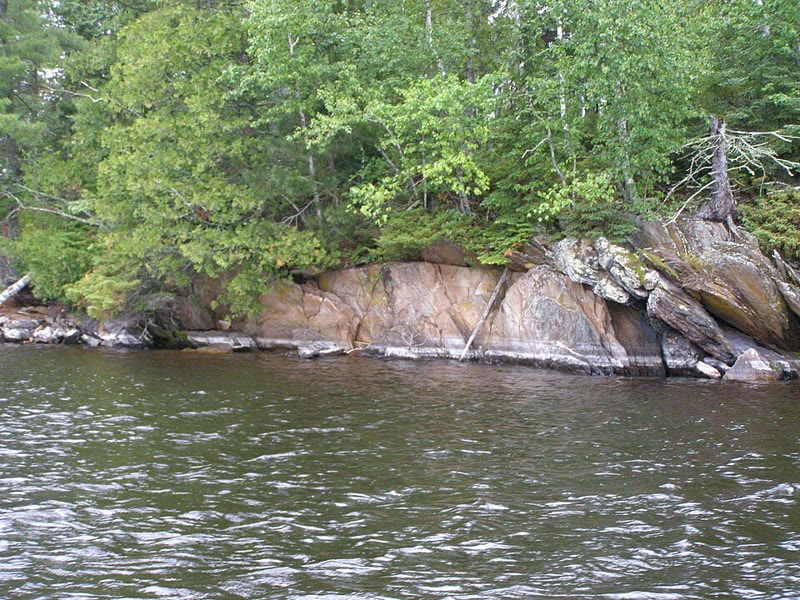
\includegraphics[height=5.0cm]{images/book2/g12-light-canadian-shield.jpg}

{\small صخور من النيس والغرانيت يتراوح عمرها بين 1 و3 مليارات سنة على شاطئ بحيرة في
كندا، جزء من النواة القديمة لأمريكا الشمالية. الصورة: كريس لايت
(\babelsublr{CC~BY-SA~4.0}).}
\end{omfigure}
% ledger: photo:g12-canadian-shield

لماذا تدوم \omterm{def:g12:continental-crust:continental-crust}{القشرة القارية}، في حين يبقى قاع المحيط فتيًا دائمًا؟
\omterm{def:g11:ocean-ridges:oceanic-lithosphere}{القشرة المحيطية} كثيفة: فهي تغوص عائدة إلى الوشاح في نطاقات \omterm{def:g11:subduction-zones:subduction}{الاندساس}،
ولا يبقى شيء منها أكثر من 200 مليون سنة بكثير. أما \omterm{def:g12:continental-crust:continental-crust}{القشرة
القارية} فأخف من أن تغوص؛ قد تبليها التعرية، أو تتمطط أو
تتجعد، لكنها تبقى على السطح. وصخور القارة
أرشيف لأربعة مليارات سنة.
% ledger: tulane:no-subduct, tulane:roots, data:b2-seafloor-age

\section{جذور الجبال}

كلما علت الجبال، ازدادت القشرة تحتها سمكًا.

\begin{definition}[جذر الجبل]\label{def:g12:continental-crust:root}
\emph{جذر}\index{جذر (السلسلة الجبلية)} السلسلة الجبلية هو
الجزء من قشرتها المُسمَّكة الذي ينزل في الوشاح تحت
مستوى \omterm{def:g11:seismic-structure:moho}{الموهو} الواقع تحت الأراضي المنخفضة المحيطة.
\end{definition}
% ledger: tulane:roots

يتنبأ نموذج إيري \omterm{def:g12:continental-crust:root}{بالجذر}: فالسلسلة المرتفعة بمقدار $h$ فوق
محيطها لها \omterm{def:g12:continental-crust:root}{جذر} $r = h\,\rho_c/(\rho_m - \rho_c)$، أي نحو خمسة أضعاف
ارتفاعها مع $\rho_c = \qty{2830}{kg/m^3}$ و$\rho_m =
\qty{3380}{kg/m^3}$ (\cref{prop:g11:lithosphere-asthenosphere:airy}). ونوعان
من القياسات يريان الجذور. فالمسوح الزلزالية تجد \omterm{def:g11:seismic-structure:moho}{الموهو} أعمق
تحت السلاسل: من 50 إلى \qty{70}{km} تحت كثير من الأحزمة الجبلية، ونحو
\qty{70}{km} تحت أجزاء من التبت. والجاذبية فوق السلاسل الجبلية أضعف مما
توحي به كتلتها المرئية: \omterm{def:g12:continental-crust:root}{فالجذر} الخفيف، القائم مكان
وشاح أكثف، يُحدث نقصًا في الكتلة في العمق، وشذوذات الجاذبية
المقيسة تتبع التضاريس وسمك القشرة الذي وجده
علم الزلازل. فالقارات تطفو، وجبالها تطفو أعلى من سواها.
% ledger: tulane:roots, karplus:tibet-moho, cm95:crust, data:prem

\section{تمارين}

\begin{exercise}[$\star$]\label{exo:g12:continental-crust:1}
انقل وأكمل \omterm{def:g12:continental-crust:continental-crust}{للقشرة القارية} \omterm{def:g11:ocean-ridges:oceanic-lithosphere}{والقشرة المحيطية}: السمك؛
الصخور الرئيسية؛ محتوى السيليكا؛ الكثافة؛ أكبر عمر.
\end{exercise}

\begin{exercise}[$\star$]\label{exo:g12:continental-crust:2}
تحوي \omterm{def:g12:continental-crust:continental-crust}{القشرة القارية} كلها \qty{60.6}{\percent} من السيليكا، وجزؤها
العلوي \qty{66.6}{\percent}. باستعمال فئات السيليكا للصخور النارية، هل
كل منهما \omterm{def:g11:igneous-rocks:felsic-mafic}{مافي} أم متوسط أم \omterm{def:g11:igneous-rocks:felsic-mafic}{فلسي}؟ سمّ صخرًا \omterm{def:g11:igneous-rocks:volcanic-plutonic}{جوفيًا} له
التركيب نفسه.
\end{exercise}

\begin{exercise}[$\star$]\label{exo:g12:continental-crust:3}
لماذا يمكن أن تغوص \omterm{def:g11:ocean-ridges:oceanic-lithosphere}{القشرة المحيطية} في الوشاح في \omterm{def:g11:subduction-zones:subduction}{نطاق اندساس}، ولا
تغوص \omterm{def:g12:continental-crust:continental-crust}{القشرة القارية}؟ أجب بالكثافات.
\end{exercise}

\begin{exercise}[$\star$]\label{exo:g12:continental-crust:4}
(1) ما \omterm{def:g12:continental-crust:craton}{الكراتون}؟ (2) ما أدنى عمر لصخور \omterm{def:g12:continental-crust:craton}{الكراتون}؟
(3) ما أنواع الصخور التي تكوّنه؟
\end{exercise}

\begin{exercise}[$\star$]\label{exo:g12:continental-crust:5}
يبلغ عمر أقدم قاع محيطي نحو 190 مليون سنة، وعمر نيس أكاستا
4.03 مليار سنة. فكم مرة يفوق عمر النيس عمر القاع؟ ولماذا لا يوجد
قاع محيطي بهذا القدم؟
\end{exercise}

\begin{exercise}[$\star\star$]\label{exo:g12:continental-crust:6}
تغطي \omterm{def:g12:continental-crust:continental-crust}{القشرة القارية} \num{210.4}~مليون~\unit{km^2}، منها
\qty{30.6}{\percent} تحت البحر. (1) ما مساحة \omterm{def:g12:continental-crust:continental-crust}{القشرة القارية}
الواقعة تحت البحر؟ (2) وما المساحة التي فوقه؟ (3) مساحة سطح الأرض
$4\pi R^2$ مع $R = \qty{6371}{km}$. فما حصة السطح التي تغطيها
\omterm{def:g12:continental-crust:continental-crust}{القشرة القارية}؟
\end{exercise}

\begin{exercise}[$\star\star$]\label{exo:g12:continental-crust:7}
احسب كتلة عمود من القشرة مقطعه \qty{1}{m^2}،
من السطح إلى \omterm{def:g11:seismic-structure:moho}{الموهو}: (1) عبر \qty{41.1}{km} من \omterm{def:g12:continental-crust:continental-crust}{القشرة
القارية} بكثافة \qty{2830}{kg/m^3}؛ (2) عبر \qty{7.1}{km} من \omterm{def:g11:ocean-ridges:oceanic-lithosphere}{القشرة المحيطية} بكثافة
\qty{3000}{kg/m^3}. (3) كم مرة يفوق الأول الثاني ثقلًا؟
\end{exercise}

\begin{exercise}[$\star\star$]\label{exo:g12:continental-crust:8}
سلسلة ترتفع \qty{2.5}{km} فوق أراضٍ منخفضة سمك قشرتها \qty{35}{km}.
مع $\rho_c = \qty{2830}{kg/m^3}$ و$\rho_m =
\qty{3380}{kg/m^3}$، احسب \omterm{def:g12:continental-crust:root}{جذرها} وسمك قشرتها. وهل
النتيجة ضمن المدى المقيس تحت الأحزمة الجبلية؟
\end{exercise}

\begin{exercise}[$\star\star$]\label{exo:g12:continental-crust:9}
من المدرج التكراري لأعمار قاع المحيط: (1) ما حصة قاع المحيط
الأحدث من 30 مليون سنة؟ (2) أي شريط من 10 ملايين سنة يضم
أكبر مساحة من القاع؟ (3) لماذا تنخفض الحصة نحو الأعمار القديمة؟
\end{exercise}

\begin{exercise}[$\star\star$]\label{exo:g12:continental-crust:10}
إذا رُسمت خريطة \omterm{def:g12:continental-crust:continental-crust}{القشرة القارية} مع أجزائها المغمورة، كان متوسط ارتفاعها
نحو \qty{120}{m}. افترض أن أجزاءها المغمورة، \qty{30.6}{\percent} من
مساحتها، تقع في المتوسط على عمق \qty{100}{m} تحت مستوى سطح البحر. فما متوسط ارتفاع
جزئها البارز؟ ولماذا تعطي التقديرات الأقدم التي لم تحسب إلا اليابسة
متوسط ارتفاع أعلى بكثير؟
\end{exercise}

\begin{exercise}[$\star\star$]\label{exo:g12:continental-crust:11}
يبلغ بئر حفر في جزيرة بعيدة في عرض محيط، تحت بضع مئات من
الأمتار من اللابات، \omterm{def:g11:ocean-ridges:gabbro}{غابرو}؛ وتضع المقاطع الزلزالية \omterm{def:g11:seismic-structure:moho}{الموهو} على عمق \qty{8}{km}.
ويبلغ بئر حفر آخر، تحت سهل واسع منبسط، النيس على عمق \qty{2}{km}،
\omterm{def:g11:seismic-structure:moho}{والموهو} على عمق \qty{38}{km}. استعمل الطريقة لتقرر أي قشرة
تقع تحت كل منهما.
\end{exercise}

\begin{exercise}[$\star\star\star$]\label{exo:g12:continental-crust:12}
ما مدى جودة تقريب القضية؟ (1) احسب الحجم الدقيق
لقشرة كروية سمكها \qty{41.1}{km} عند سطح كرة نصف
قطرها \qty{6371}{km}، $\tfrac{4}{3}\pi\bigl(R^3 - (R - H)^3\bigr)$،
والحجم التقريبي، $4\pi R^2 H$. (2) ما الفرق النسبي؟ وقارنه
بالنسبة $H/R$.
\end{exercise}

\begin{exercise}[$\star\star\star$]\label{exo:g12:continental-crust:13}
افترض أن الثلث العلوي من \omterm{def:g12:continental-crust:continental-crust}{القشرة القارية}، كتلةً، يحوي
\qty{66.6}{\percent} من السيليكا، والقشرة كلها \qty{60.6}{\percent}. (1)
ما محتوى الثلثين السفليين من السيليكا؟ (2) أي فئة من
الصخور النارية يوافق؟ (3) ماذا يقول ذلك عن \omterm{def:g12:continental-crust:continental-crust}{القشرة
القارية} العميقة؟
\end{exercise}

\begin{exercise}[$\star\star\star$]\label{exo:g12:continental-crust:14}
افترض أن \omterm{def:g11:ocean-ridges:oceanic-lithosphere}{قشرة محيطية} جديدة تتكوّن عند الظهرات بمعدل نحو \qty{3}{km^2} في
السنة، وأن قاع المحيط يغطي نحو \num{300}~مليون~\unit{km^2}. (1)
كم ستستغرق الظهرات لتصنع مساحة تساوي قاع المحيط
كله؟ (2) قارن ذلك بأعمار قاع المحيط. (3) ماذا يجب أن يحدث
للقاع القديم؟
\end{exercise}

\begin{exercise}[$\star\star\star$]\label{exo:g12:continental-crust:15}
افترض أن \omterm{def:g12:continental-crust:continental-crust}{القشرة القارية} كلها، \qty{8.6e9}{km^3}، تكوّنت بمعدل
ثابت منذ 4.0 مليار سنة. (1) احسب المعدل بالكيلومترات المكعبة في
السنة. (2) تُظهر زركونات تلال جاك أن بعض القشرة كان موجودًا قبل
4.4 مليار سنة. فهل يلائم المعدل الثابت عالمًا ربما تكوّن فيه معظم
القشرة مبكرًا، أم متأخرًا؟ وماذا يمكن أن تخبرنا به أقدم الصخور، وماذا
لا تستطيع، علمًا بأن القشرة القديمة قد تتآكل أو يُعاد تدويرها؟
\end{exercise}

\section{مسألة: ما وزن القشرة القارية؟}

\begin{problem}[{مسألة نهاية الأسبوع --- كتلة القارات}]
\label{pb:g12:continental-crust:1}
% ledger: cogley84:continents, cm95:crust, earth:mass, earth:Rmean, earth:density, white92:crust
% values: 4 pi R^2 = 5.1006e8 km2; V = 210.4e6 x 41.1 = 8.647e9 km3; m = 2.447e22 kg; m/M = 0.410 %
تغطي \omterm{def:g12:continental-crust:continental-crust}{القشرة القارية} \num{210.4}~مليون~\unit{km^2} (بما فيها الأجزاء
المغمورة). وتعطيها المسوح الزلزالية سمكًا متوسطًا قدره \qty{41.1}{km}
ومتوسط كثافة قدره \qty{2830}{kg/m^3}. ونصف قطر الأرض المتوسط
\qty{6371}{km}، وكتلتها \qty{5.9722e24}{kg}، ومتوسط كثافتها
\qty{5513}{kg/m^3}.

\medskip
\noindent\textbf{الجزء الأول --- المساحة.}
\begin{enumerate}
  \item احسب مساحة سطح الأرض، $4\pi R^2$، بوحدة
        \unit{km^2}.
  \item ما حصتها التي تغطيها \omterm{def:g12:continental-crust:continental-crust}{القشرة القارية}؟
  \item يقع \qty{30.6}{\percent} من \omterm{def:g12:continental-crust:continental-crust}{القشرة القارية} تحت البحر.
        فما مساحة ذلك؟
  \item ما المساحة الباقية من سطح الأرض \omterm{def:g11:ocean-ridges:oceanic-lithosphere}{للقشرة المحيطية}،
        بافتراض أن الباقي كله محيطي؟
  \item لماذا \omterm{def:g12:continental-crust:continental-crust}{القشرة القارية} أوسع من اليابسة؟
\end{enumerate}

\medskip
\noindent\textbf{الجزء الثاني --- السمك والحجم.}
\begin{enumerate}[resume]
  \item لماذا يمكن حساب الحجم بضرب المساحة في السمك، مع أن
        القشرة تقع على كرة؟
  \item احسب حجم \omterm{def:g12:continental-crust:continental-crust}{القشرة القارية} بوحدة \unit{km^3}.
  \item حوّله إلى \unit{m^3}.
  \item تقدير آخر للسمك المتوسط هو \qty{36}{km}. فأي
        حجم يعطي؟
  \item بكم في المئة يختلف الحجمان؟
\end{enumerate}

\medskip
\noindent\textbf{الجزء الثالث --- الكثافة والكتلة.}
\begin{enumerate}[resume]
  \item احسب كتلة \omterm{def:g12:continental-crust:continental-crust}{القشرة القارية} بسمك \qty{41.1}{km}.
  \item احسب كتلة عمود مقطعه \qty{1}{m^2} عبر \omterm{def:g12:continental-crust:continental-crust}{القشرة
        القارية}.
  \item احسب كتلة \omterm{def:g11:ocean-ridges:oceanic-lithosphere}{القشرة المحيطية}: المساحة من السؤال~4،
        والسمك \qty{7.1}{km}، والكثافة \qty{3000}{kg/m^3}.
  \item أيهما أثقل، وبكم مرة؟ ولماذا، مع أنها تغطي مساحة
        أقل؟
  \item لماذا \omterm{def:g12:continental-crust:continental-crust}{القشرة القارية} أقل كثافة من \omterm{def:g11:ocean-ridges:oceanic-lithosphere}{القشرة المحيطية}؟
\end{enumerate}

\medskip
\noindent\textbf{الجزء الرابع --- مقارنةً بالأرض.}
\begin{enumerate}[resume]
  \item اقسم كتلة السؤال~11 على كتلة الأرض.
  \item تحقق من النتيجة بقضية الطبقات الرقيقة.
  \item ما حصة \omterm{def:g11:ocean-ridges:oceanic-lithosphere}{القشرة المحيطية} من كتلة الأرض؟
  \item تحوي \omterm{def:g12:continental-crust:continental-crust}{القشرة القارية} الصخور الوحيدة الأقدم من نحو 200
        مليون سنة. فما حصة كتلة الأرض التي تحمل سجل
        تاريخها كله تقريبًا؟
  \item استنتج: ما حصة \omterm{def:g12:continental-crust:continental-crust}{القشرة القارية} من كتلة الأرض؟
\end{enumerate}
\end{problem}
